% Same conference class and column geometry as template.tex.
\documentclass[conference]{IEEEtran}
\usepackage{cite}
\usepackage{amsmath,amssymb,amsfonts}
\usepackage{graphicx}
\usepackage{booktabs,tabularx}
\usepackage{xcolor}
\usepackage{microtype}
\usepackage{balance}
\usepackage[hidelinks]{hyperref}
\hypersetup{pdftitle={How Much Should a Return Forecast Forget? Adaptive Bayesian Updating Across Asset Classes},
  pdfauthor={Rahul Sunilkumar},pdfsubject={Fall 2025 research paper},
  pdfkeywords={Bayesian updating, return forecasting, forgetting factor}}
\graphicspath{{figures/}{writeup/figures/}}
\newcommand{\E}{\mathbb{E}}
\newcommand{\sgn}{\operatorname{sign}}
\date{Fall 2025}

\begin{document}
\raggedbottom

\title{How Much Should a Return Forecast Forget?\\
Adaptive Bayesian Updating Across Asset Classes}
\author{\IEEEauthorblockN{Rahul Sunilkumar}
\IEEEauthorblockA{University of Virginia\\
Charlottesville, Virginia\\
Fall 2025}}
\maketitle

\begin{abstract}
How much history should a return forecast retain? I compare a Gaussian Bayesian mean update with six simple rules on daily returns for 24 exchange-traded funds from 2010 through 2024. The default model achieves 51.36 percent directional accuracy but an average trading Sharpe of only 0.012, compared with 0.204 for a first-order autoregression. Predicting zero gives lower root mean squared error on every asset. Performance varies across assets and weakens in high volatility. In the parameter sweep, no forgetting produces the highest average Sharpe at every tested window. These results suggest that retaining information helped in this sample, although they do not establish why or demonstrate reliable market-timing ability.

\end{abstract}

\begin{IEEEkeywords}
Bayesian updating, return forecasting, forgetting factor, volatility, walk-forward evaluation
\end{IEEEkeywords}

\section{Introduction}
A short return window responds quickly but can mistake noise for a change in the mean. A long window is steadier but retains information that may no longer matter. Bayesian updating makes this tradeoff explicit by weighting the current estimate and each new observation according to their uncertainty.

I wanted to see whether this mechanism improves on ordinary averages, and whether forgetting helps when conditions change. Each asset is forecast from its own return history. The result led me in the opposite direction: removing forgetting improved performance. That made me look more closely at what the forgetting factor actually changes, and what the results can tell us about it.

\section{The Bayesian Update}
\subsection{A Working Model for the Mean}
Let $P_t$ denote adjusted closing price and define the simple daily return
\begin{equation}
 r_t = \frac{P_t}{P_{t-1}}-1.
\end{equation}
After observing $r_t$, the task is to forecast $r_{t+1}$.

The model treats the latest return as a noisy observation of a local mean $\mu_t$. Immediately before assimilating it, write
\begin{equation}
 \mu_t\sim\mathcal N(m_{t-1},R_t),\qquad
 r_t\mid\mu_t,V_t\sim\mathcal N(\mu_t,V_t).
 \label{eq:model}
\end{equation}
Here $R_t$ measures uncertainty about the mean; $V_t$ measures variability of individual returns.

I estimate $V_t$ from the latest $w$ returns, whose sample mean is $\bar r_{t,w}$:
\begin{equation}
 V_t=\max\left\{\frac{\sum_{j=t-w+1}^{t}(r_j-\bar r_{t,w})^2}{w-1},10^{-10}\right\}.
 \label{eq:variance}
\end{equation}
The floor avoids division by zero. The estimated $V_t$ includes $r_t$ and is treated as known, so this is a plug-in conjugate update rather than a joint model of mean and variance \cite{murphy}.

Multiplying the prior and likelihood gives
\begin{equation}
 p(\mu_t\mid r_t)\propto
 \exp\left[-\frac12\left\{
 \frac{(\mu_t-m_{t-1})^2}{R_t}
 +\frac{(r_t-\mu_t)^2}{V_t}\right\}\right].
\end{equation}
Collecting the quadratic and linear terms in $\mu_t$ yields a normal posterior with variance $C_t$ and mean $m_t$:
\begin{align}
 C_t&=\left(R_t^{-1}+V_t^{-1}\right)^{-1},\label{eq:postvar}\\
 m_t&=C_t\left(\frac{m_{t-1}}{R_t}+\frac{r_t}{V_t}\right).
 \label{eq:postmean}
\end{align}
Thus precisions, the reciprocals of variances, add. The code returns $\hat r_{t+1}=m_t$.

The update is easier to make sense of in this form:
\begin{equation}
 m_t=m_{t-1}+K_t(r_t-m_{t-1}),\qquad
 K_t=\frac{R_t}{R_t+V_t}.
 \label{eq:gain}
\end{equation}
The gain $K_t$ is the fraction of the forecast error absorbed into the new estimate. Holding $R_t$ fixed, larger return variance lowers the gain. 

\subsection{Forgetting and Effective Memory}
Without an allowance for change, repeated observations keep reducing uncertainty. The implementation carries the posterior mean forward and discounts its precision:
\begin{equation}
 R_{t+1}=\frac{C_t}{\delta},\qquad 0<\delta\leq1.
 \label{eq:discount}
\end{equation}
Variance discounting has a long history in Bayesian forecasting \cite{ameen}. Here $\delta=1$ adds no uncertainty, while smaller values allow subsequent observations to move the estimate more.

With constant $V_t=V$ and $\delta<1$, solving the steady-state equation $R=RV/[\delta(R+V)]$ gives
\begin{equation}
 R^*=\frac{1-\delta}{\delta}V,\qquad
 C^*=(1-\delta)V,\qquad K^*=1-\delta.
 \label{eq:steady}
\end{equation}
The mean update then approaches exponential smoothing:
\begin{equation}
 m_t=\delta m_{t-1}+(1-\delta)r_t.
\end{equation}
At the default $\delta=0.98$, the limiting gain is 2\%, with weight half-life $\log(1/2)/\log\delta\approx34.3$ trading days. In the experiment, changing $V_t$ makes the gain vary. The window estimates observation variance; it does not truncate the mean's memory.

When $\delta=1$, the update has a different limiting behavior. Starting the recursion at observation $t_0$, repeated substitution gives
\begin{equation}
 m_t=\frac{m_0/R_{t_0}+\sum_{j=t_0}^{t}r_j/V_j}
 {1/R_{t_0}+\sum_{j=t_0}^{t}1/V_j}.
 \label{eq:noforget}
\end{equation}
This is an accumulating precision-weighted average. It is not generally the ordinary expanding mean, since observations from low-variance windows receive greater weight.

\subsection{Initialization}
The first $p$ returns initialize $m_0$ to their sample mean and $R_{t_0}$ to their sample variance divided by $p$, floored at $10^{-10}$. The default uses $p=w=50$ and $\delta=0.98$. Forecasting begins after 300 observations: the original code initializes from the first 50 and then assimilates $r_{300}$, without sequentially updating or discounting across the intervening history. The effect of this initialization choice is not evaluated separately.

\section{Data and Experimental Design}
\subsection{Assets and Forecast Timing}
The saved data contain adjusted daily prices from January 4, 2010 through December 30, 2024, downloaded with \texttt{yfinance} \cite{yfinance}. Table~\ref{tab:universe} lists the 24 analyzed funds; VXX was downloaded but excluded.

\begin{table}[t]
\caption{Asset universe}
\label{tab:universe}
\centering\footnotesize
\begin{tabularx}{\columnwidth}{@{}lX@{}}
\toprule
Asset class & Tickers\\
\midrule
U.S. equity & SPY, QQQ, IWM, DIA, XLF, XLE, XLK, XLV, XLU, XLP\\
International equity & EFA, EEM, EWJ, FXI\\
Fixed income & TLT, IEF, LQD, HYG, TIP\\
Commodities & GLD, SLV, USO, DBC\\
Real estate & VNQ\\
\bottomrule
\end{tabularx}
\end{table}

Each series has 3,772 nonmissing returns. Reserving the first 300 as history leaves 3,472 forecast dates per asset, from March 15, 2011 through December 30, 2024. The walk-forward evaluator passes only earlier returns to each model and resets its state between assets. Trading assumes positions can be formed at the preceding close without execution delay.

\subsection{Baseline Forecasts}
The zero rule predicts $\hat r_{t+1}=0$. The rule called \texttt{Random Walk} in the code predicts $\hat r_{t+1}=r_t$. I call the latter \emph{last return} below: it assumes persistence in returns, whereas a driftless random walk in price would motivate a zero expected return.

The rolling means use $\hat r_{t+1}=w^{-1}\sum_{j=0}^{w-1}r_{t-j}$ for $w=50$ and $250$. The exponentially weighted moving average (EWMA) uses all available history, normalized at each forecast:
\begin{equation}
 \hat r_{t+1}=\frac{\sum_{j=0}^{t-1}\lambda^j r_{t-j}}
 {\sum_{j=0}^{t-1}\lambda^j},\qquad \lambda=2^{-1/20}.
\end{equation}
Its 20-day half-life is shorter than the Bayesian default's constant-variance half-life, so these are not memory-matched comparisons.

The first-order autoregression, AR(1), fits $r_j=a+br_{j-1}+\epsilon_j$ by least squares on 250 lagged pairs and predicts $\hat r_{t+1}=\hat a_t+\hat b_t r_t$. Unlike last return, it can estimate either positive or negative dependence.

\subsection{Forecast and Trading Scores}
Forecast error is measured by root mean squared error (RMSE) and mean absolute error (MAE). Directional accuracy is the fraction of matching signs, excluding zero forecasts and zero returns.

For trading, positions and daily strategy returns are
\begin{equation}
 q_t=\sgn(\hat r_t),\qquad g_t=q_t r_t.
 \label{eq:trading}
\end{equation}
A tiny positive forecast therefore takes a full long position. Posterior uncertainty does not affect position size.

Annualized Sharpe is
\begin{equation}
 S=\sqrt{252}\frac{\bar g}{s_g}.
 \label{eq:sharpe}
\end{equation}
I also report annualized compounded growth from the daily strategy returns.
Here $s_g$ is the sample standard deviation. The ratio uses a zero cash benchmark and omits financing, borrowing, and transaction costs; the $\sqrt{252}$ scaling is a convention that need not hold under serial dependence \cite{sharpe}. All aggregates average the 24 asset-level scores, rather than describing a combined portfolio. The zero rule has no reported directional or trading scores.

\section{Results}
\subsection{Small Forecasts, Small Differences in Error}
Table~\ref{tab:main} shows that zero has the lowest average RMSE. The default Bayesian model is only 0.533 basis points worse per day, but fails to beat zero on any asset. The 250-day rolling mean has the lowest average MAE.

\begin{table*}[t]
\caption{Walk-forward results, averaged over 24 assets}
\label{tab:main}
\centering\small
\begin{tabular}{lrrrrr}
\toprule
Method & RMSE (bp/day) & MAE (bp/day) & Hit rate (\%) & Annualized Sharpe & Compound growth (\%/yr)\\
\midrule
Zero & \textbf{115.940} & 80.526 & --- & --- & ---\\
Last return & 168.175 & 116.566 & 49.30 & $-0.173$ & $-4.92$\\
Rolling mean, 50d & 117.144 & 81.161 & 51.27 & 0.013 & $-1.87$\\
Rolling mean, 250d & 116.122 & \textbf{80.425} & \textbf{52.28} & 0.160 & 0.57\\
EWMA, half-life 20d & 117.107 & 81.147 & 51.08 & 0.019 & $-2.21$\\
AR(1), 250d & 116.350 & 80.624 & 51.99 & \textbf{0.204} & \textbf{1.58}\\
Bayesian, $w=50$, $\delta=0.98$ & 116.472 & 80.766 & 51.36 & 0.012 & $-1.88$\\
\bottomrule
\end{tabular}
\vspace{3pt}

\parbox{0.96\textwidth}{\footnotesize Each method has 3,472 forecast dates per asset. One basis point (bp) is $10^{-4}$ in decimal return. Trading scores use a zero cash rate and omit costs. Bold values mark the best aggregate in each column; they do not indicate statistical significance.}
\end{table*}

At first glance, that small error gap looks reassuring. For any forecast $f$, its squared-error difference from predicting zero is exactly
\begin{equation}
 (r-f)^2-r^2=f^2-2rf.
 \label{eq:loss}
\end{equation}
A nonzero estimate improves expected squared error only if its alignment with the next return is large enough to offset its own squared magnitude. Shrinking forecasts toward zero can keep errors small without extracting much useful signal.

\subsection{Directional Accuracy Is Not Profitability}
The Bayesian hit rate is 51.36\%, yet its average Sharpe is 0.012 and its average compound growth is $-1.88$\% per year. The 250-day rolling mean gets direction right more often than AR(1), but AR(1) has the larger average Sharpe.

Hit rate counts days; trading returns weight them by the size of the move. A few large misses can outweigh getting the sign right more often. Compounding further penalizes volatility: for small returns, $\E[\log(1+g)]\approx\E[g]-\E[g^2]/2$.

\subsection{The Aggregate Hides Asset Differences}
The heatmap in Fig.~\ref{fig:assets} shows substantial variation across assets. Bayesian mean Sharpe is positive in fixed income (0.236) and commodities (0.139), but negative in U.S. equity ($-0.082$), international equity ($-0.060$), and VNQ ($-0.394$), the sole real-estate fund. Even in the positive groups, the 250-day rolling mean has higher class-average Sharpes: 0.291 and 0.179, respectively.

\begin{figure}[t]
\centering
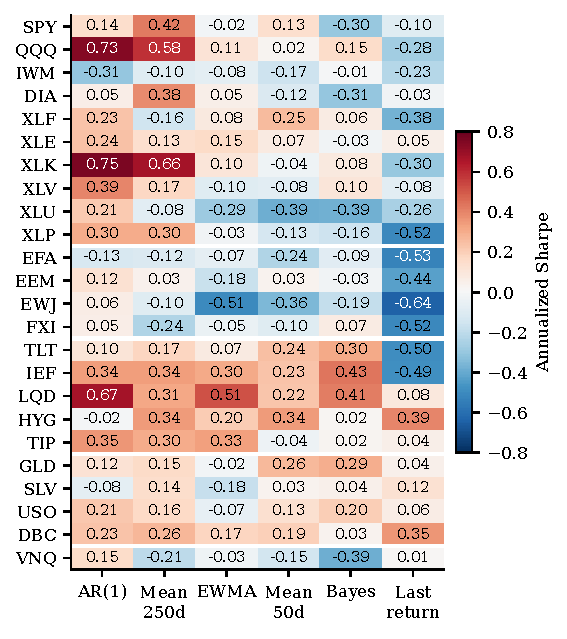
\includegraphics[width=\columnwidth]{asset_sharpes.pdf}
\caption{Asset-level trading Sharpes. Groups from top to bottom are U.S. equity, international equity, fixed income, commodities, and real estate. ``Bayes'' uses the default settings; ``Last return'' is the code's Random Walk rule.}
\label{fig:assets}
\end{figure}

\subsection{Volatility Changes the Picture}
For each asset, I split days using the preceding 20 returns' standard deviation and its full-sample median. These are retrospective volatility groups. Their Sharpes use the same annualization as the full sample, not the calendar-time performance of a regime-switching strategy.

Bayesian average Sharpe falls from 0.382 in low volatility to $-0.206$ in high volatility (Fig.~\ref{fig:regimes}), much like the 50-day rolling mean. AR(1) remains positive in both groups. Equation~\eqref{eq:gain} suggests a possible explanation: higher observation variance can suppress revisions just as conditions change, while \eqref{eq:trading} leaves exposure at full size. Adapting the forecast's gain does not automatically adapt its trading risk.

\begin{figure}[t]
\centering
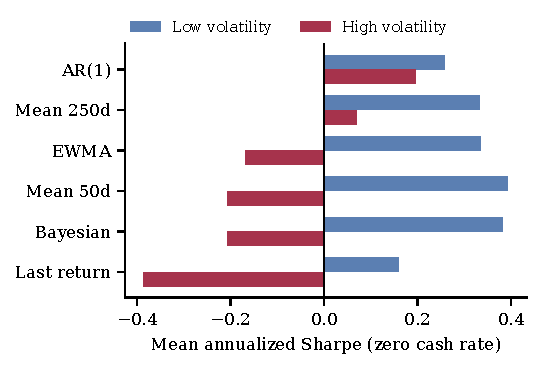
\includegraphics[width=\columnwidth]{regimes.pdf}
\caption{Mean asset-level Sharpe conditional on lagged volatility. All six active rules perform worse in the high-volatility group. The default Bayesian model's low-volatility result does not persist across regimes.}
\label{fig:regimes}
\end{figure}

\section{Sensitivity to Forgetting and Window Size}
\label{sec:sensitivity}
The parameter sweep tests $w\in\{10,25,50,100,250\}$ and $\delta\in\{0.95,0.98,0.99,1\}$. Table~\ref{tab:sweep} contains the average Sharpes. At every window, no forgetting wins. Most settings with $\delta=0.95$ are near zero or negative.

\begin{table}[t]
\caption{Mean Bayesian Sharpe across parameter settings}
\label{tab:sweep}
\centering\footnotesize
\begin{tabular}{@{}lrrrrr@{}}
\toprule
 & \multicolumn{5}{c}{Variance window $w$ (trading days)}\\
\cmidrule(l){2-6}
$\delta$ & 10 & 25 & 50 & 100 & 250\\
\midrule
0.95 & $-0.031$ & 0.016 & $-0.045$ & $-0.015$ & 0.053\\
0.98 & 0.070 & 0.003 & 0.012 & 0.012 & 0.043\\
0.99 & 0.194 & 0.104 & 0.062 & 0.089 & 0.118\\
1.00 & 0.395 & 0.365 & 0.317 & 0.286 & 0.397\\
\bottomrule
\end{tabular}
\end{table}

At $w=50$, increasing $\delta$ from 0.98 to 1 raises average Sharpe from 0.012 to 0.317. The strongest observed settings use no forgetting with windows of 10 and 250 days, at 0.395 and 0.397. Shorter memory does not appear to help this model in the sample.

Equation~\eqref{eq:noforget} offers one possible interpretation: retaining observations can stabilize a mean estimate when daily returns are noisy. But the sweep does not measure whether the improvement comes from better timing, persistent exposure, or another feature of the return history. I would be careful about giving the result a stronger explanation than the experiment supports.

There is also a catch when comparing windows. The sweep sets $p=\max(w,50)$ and starts forecasting after $\max(300,2w)$ returns. The 250-day setting therefore uses a longer prior sample and only 3,272 evaluation dates. Forgetting factors are compared on common dates within each window, but the ranking across windows cannot be attributed to window size alone.

\section{Limits and Next Steps}
\balance
The universe is fixed retrospectively and contains overlapping exposures. Parameters were compared on the same period used to report performance, with no final holdout or formal test of the differences between methods. The rankings describe this sample rather than an independently validated trading strategy.

The model treats estimated return variance as known and uses only the forecast sign to trade. Its initialization also skips sequential updates through part of the available history. These choices limit what the results say about Bayesian forecasting more broadly.

A next step would be to hold prior length and evaluation dates fixed across windows and compare against an always-long position. An EWMA with a roughly 34-day half-life would help distinguish variable gains from ordinary smoothing. Those comparisons, and testing on unused dates, would make it easier to tell what the Bayesian update contributes.

\section{Conclusion}
The default Bayesian model produces a smooth mean estimate, but loses to zero on RMSE for every asset and performs poorly as a trading signal, especially in high volatility. AR(1) has the highest average trading Sharpe among the original methods, while the 250-day rolling mean has the highest directional accuracy.

The result I find most interesting is that no forgetting performs best at every tested window. Retaining information appears more useful here than reacting more strongly to recent returns. That tells me something about this update rule in this sample; it does not settle why the improvement occurs or whether it would persist in a new period.

\section*{Reproducibility}
Source and replication scripts are in the GitHub repository \cite{repository}. With NumPy, pandas, and Matplotlib installed, use the saved returns in \texttt{data/} and run \texttt{run\_analysis.py}, \texttt{window\_sweep.py}, and \texttt{make\_plots.py} from the repository root, in that order. These reproduce the scores, parameter sweep, and original plots. The paper's figures show the same results with adjusted formatting. To download data again, run \texttt{fetch.py} with yfinance installed; later data revisions may change the values.

\begin{thebibliography}{00}
\bibitem{murphy}
K. P. Murphy, ``Conjugate Bayesian analysis of the Gaussian distribution,'' technical report, Oct. 2007. [Online]. Available: \url{https://www.cs.ubc.ca/~murphyk/Papers/bayesGauss.pdf}

\bibitem{ameen}
J. R. M. Ameen and P. J. Harrison, ``Normal discount Bayesian models,'' in \emph{Bayesian Statistics 2}, J. M. Bernardo, M. H. DeGroot, D. V. Lindley, and A. F. M. Smith, Eds. Amsterdam: North-Holland, 1985, pp. 271--298. [Online]. Available: \url{https://www2.stat.duke.edu/~mw/MWextrapubs/BayesStatist2.pdf}

\bibitem{yfinance}
R. Aroussi, ``yfinance: Download market data from Yahoo! Finance,'' software documentation. [Online]. Available: \url{https://ranaroussi.github.io/yfinance/reference/api/yfinance.download.html}

\bibitem{sharpe}
W. F. Sharpe, ``The Sharpe ratio,'' \emph{The Journal of Portfolio Management}, vol. 21, no. 1, pp. 49--58, Fall 1994. [Online]. Available: \url{https://web.stanford.edu/~wfsharpe/art/sr/sr.htm}
\bibitem{repository}
R. Sunilkumar, ``Bayesian updating,'' GitHub repository. [Online]. Available: \url{https://github.com/rahulsunilkumar/bayesian-updating}
\end{thebibliography}

\end{document}
